\section*{Question 1}
\subsection*{(c)}
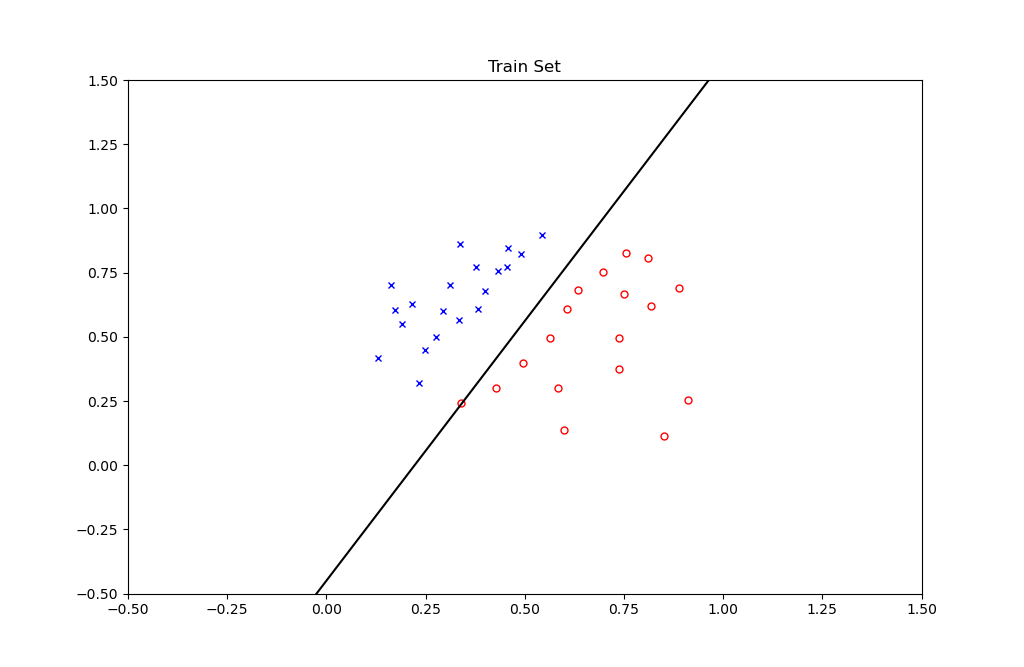
\includegraphics[width=0.5\textwidth]{q1_leastSquare_linear_classifier_python/Figure_1.png}
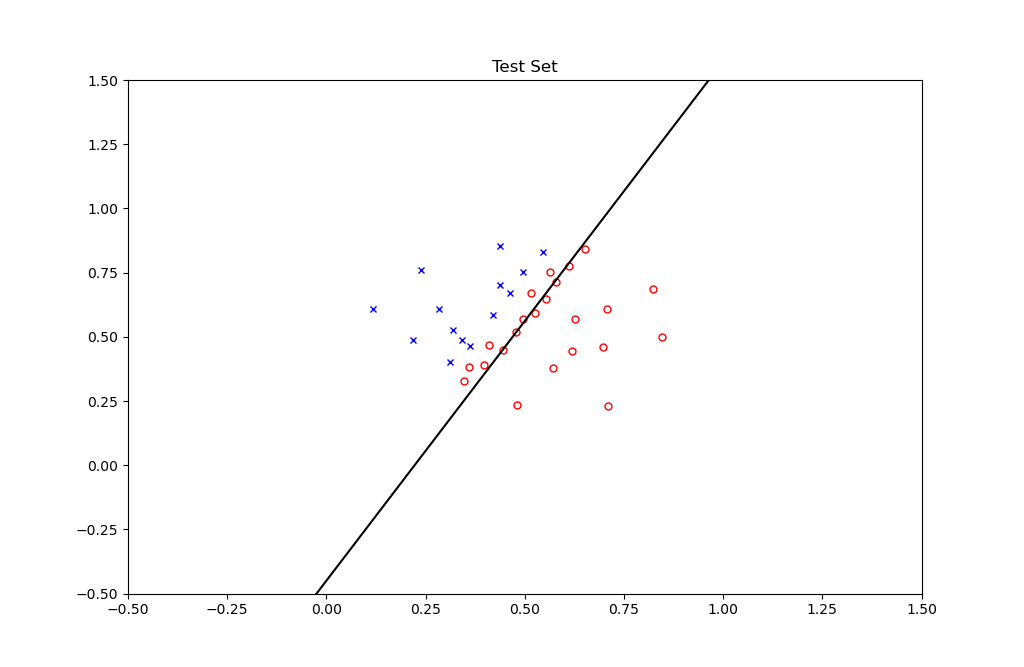
\includegraphics[width=0.5\textwidth]{q1_leastSquare_linear_classifier_python/Figure_2.png}

Accuracy on train set: $0.9736842105263158$ \\
Accuracy on test set: $0.7837837837837838$

We can see, that not even for the training data the resulting classifier fully classifies the data. Especially, we can see that the margin between classifier and the data of the two categories is not maximal, thus reducing generalization. This is also shown using the test set.


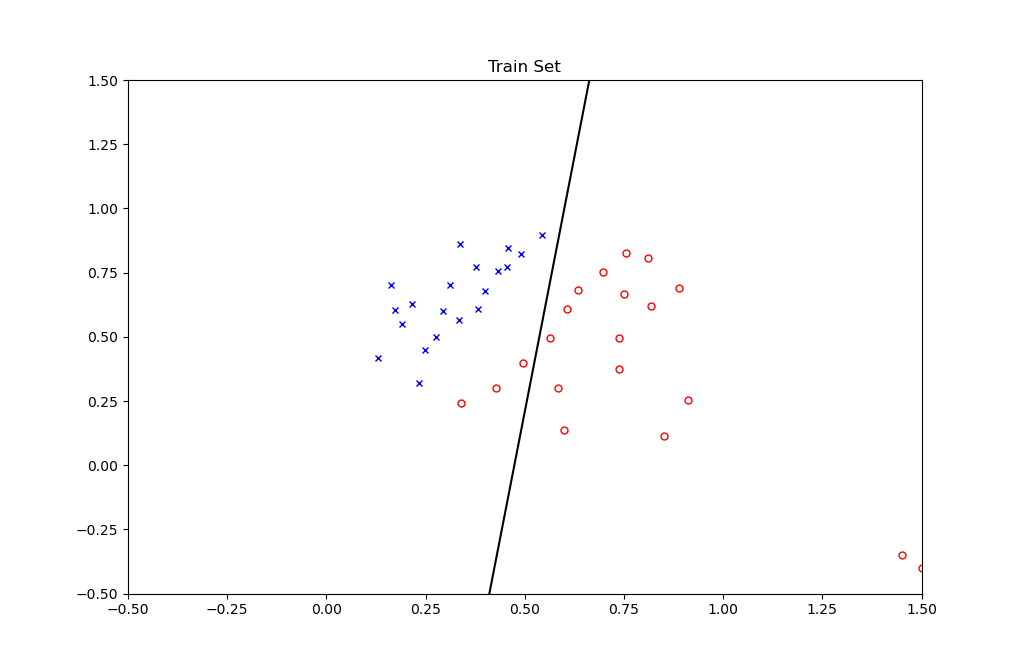
\includegraphics[width=0.5\textwidth]{q1_leastSquare_linear_classifier_python/Figure_3.png}
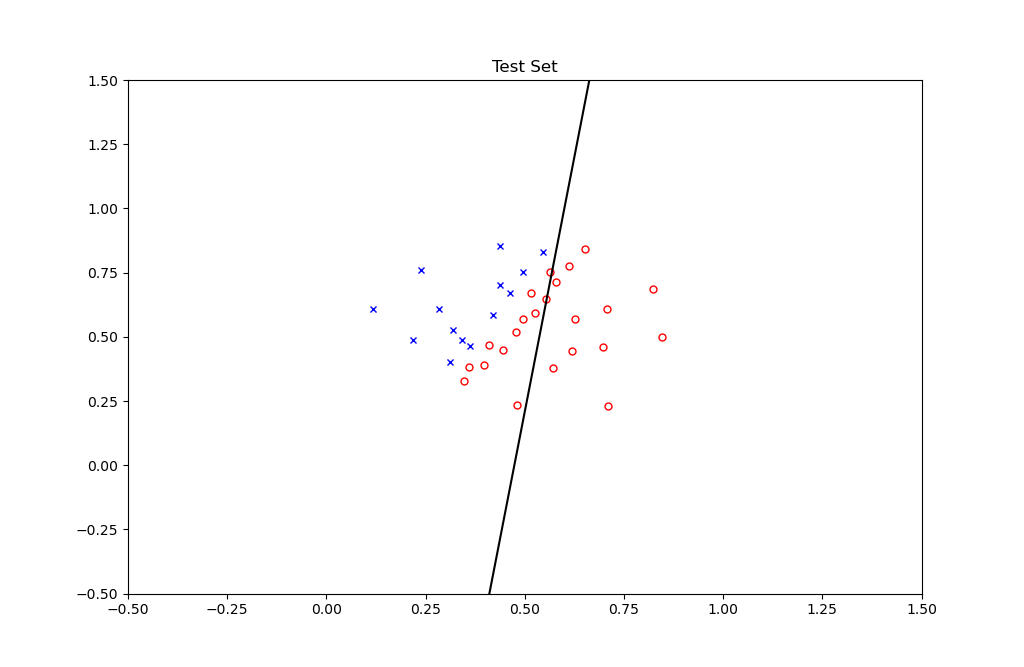
\includegraphics[width=0.5\textwidth]{q1_leastSquare_linear_classifier_python/Figure_4.png}


Adding outliers...
Accuracy on train set: $0.925$ \\
Accuracy on test set: $0.6756756756756757$

We can see that adding outliers further disrupts the accuracy of the classifier, which is to be expected with a least-squares classifier as discussed in the lecture.
